\begin{frame}
	\titlepage
\end{frame}

\begin{frame}{平面曲线的曲率}
	\linespread{1.5}
	\begin{columns}
		\column{.5\textwidth}
			\vspace{-2cm}
			\begin{itemize}
		      \item {\bf 平面曲线的曲率概念}
		      \item {\bf 曲率的计算公式}
		      \item {\bf 曲率圆与曲率的应用}
		    \end{itemize}
		\column{.5\textwidth}
			\vspace{2cm}
			\resizebox{!}{5cm}{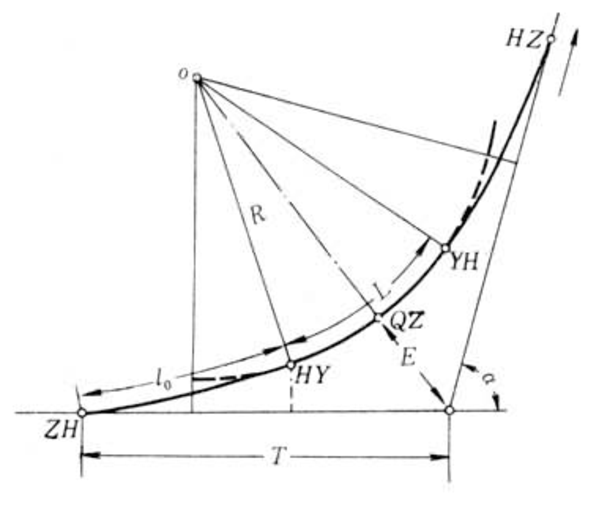
\includegraphics{./images/tcs.pdf}}
	\end{columns}
\end{frame}

\begin{frame}{铁路的设计}
	\linespread{1.2}
	\begin{center}
		\resizebox{!}{7cm}{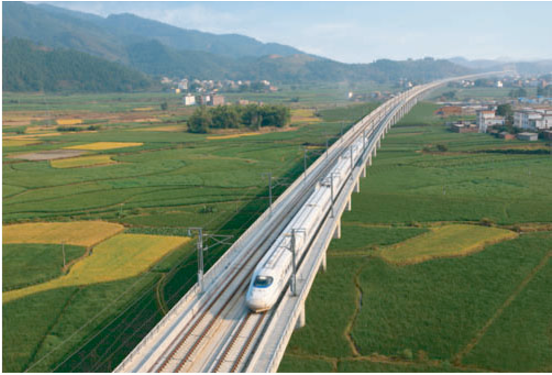
\includegraphics{./images/rw1.pdf}}
	\end{center}
\end{frame}

\begin{frame}{复习与回顾}
	\linespread{1.5}
% 	\begin{center}
% 		\ba{一元函数的导数/微分与平面曲线的几何特征}
% 	\end{center}
% 	
	\ba{如何刻画一条平面曲线的几何特征?}
% 	\ba{平面曲线的几何特征与一元函数的导数和微分:}
	
	\begin{itemize}
	  \item {\bf 切线斜率:}一阶导数
	  \item {\bf 凹凸性:}二阶导数
	  \item {\bf 长度:}弧微分\pause
	  \item {\bf 弯曲程度:}{\b 曲率}
	\end{itemize}
\end{frame}

\section{曲率}

\subsection{曲率的概念}

\begin{frame}{曲率}
	\linespread{1.2}
	\centerline{\ba{如何刻画曲线的弯曲程度?}}
	\pause
	\begin{columns}
		\column{.5\textwidth}
			\begin{center}
				\vspace{-1em}
				{\resizebox{!}{5.5cm}{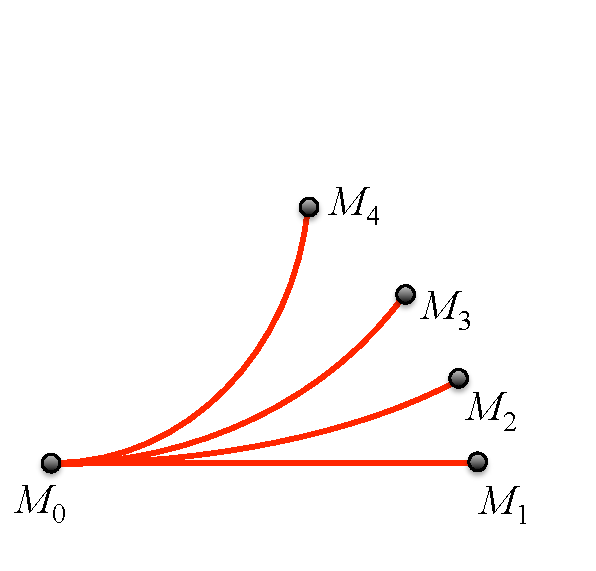
\includegraphics{./images/curves/c106.pdf}}}

				\vspace{-1em}\invisible<1->{{\b 长度相同的曲线,切线

				转角越大弯曲程度越大}}
			\end{center}
		\column{.5\textwidth}
	\end{columns}
\end{frame}

\begin{frame}{曲率}
	\linespread{1.2}
	\centerline{\ba{如何刻画曲线的弯曲程度?}}

	\begin{columns}
		\column{.5\textwidth}
			\begin{center}
				\vspace{-1em}
				{\resizebox{!}{5.5cm}{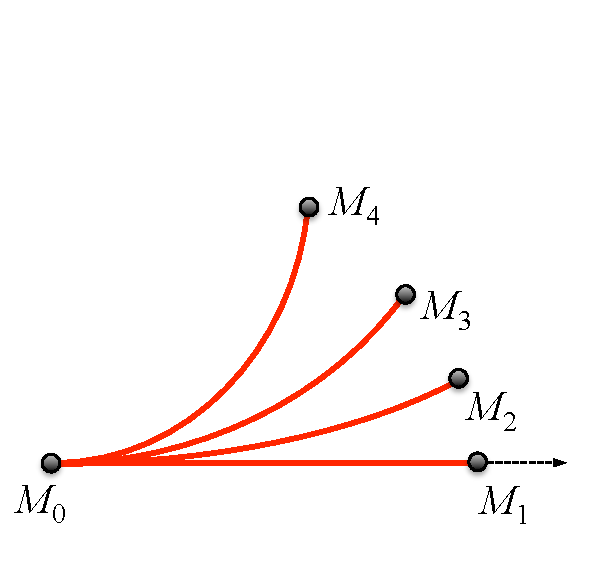
\includegraphics{./images/curves/c105.pdf}}}

				\vspace{-1em}\invisible<1->{{\b 长度相同的曲线,切线

				转角越大弯曲程度越大}}
			\end{center}
		\column{.5\textwidth}
	\end{columns}
\end{frame}

\begin{frame}{曲率}
	\linespread{1.2}
	\centerline{\ba{如何刻画曲线的弯曲程度?}}

	\begin{columns}
		\column{.5\textwidth}
			\begin{center}
				\vspace{-1em}
				{\resizebox{!}{5.5cm}{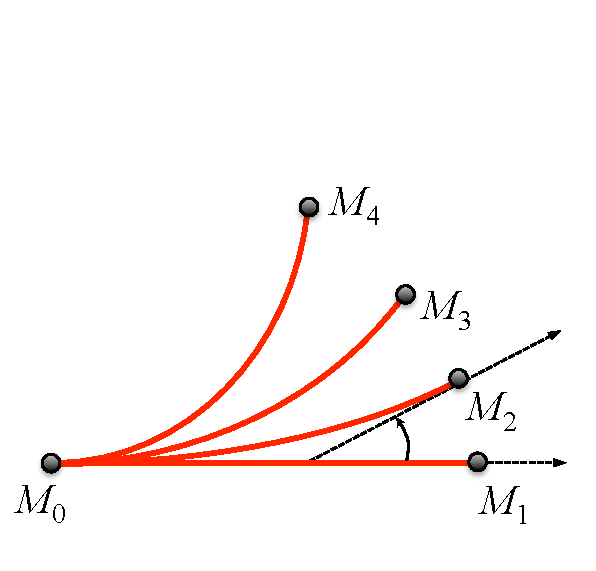
\includegraphics{./images/curves/c104.pdf}}}

				\vspace{-1em}\invisible<1->{{\b 长度相同的曲线,切线

				转角越大弯曲程度越大}}
			\end{center}
		\column{.5\textwidth}
	\end{columns}
\end{frame}

\begin{frame}{曲率}
	\linespread{1.2}
	\centerline{\ba{如何刻画曲线的弯曲程度?}}

	\begin{columns}
		\column{.5\textwidth}
			\begin{center}
				\vspace{-1em}
				{\resizebox{!}{5.5cm}{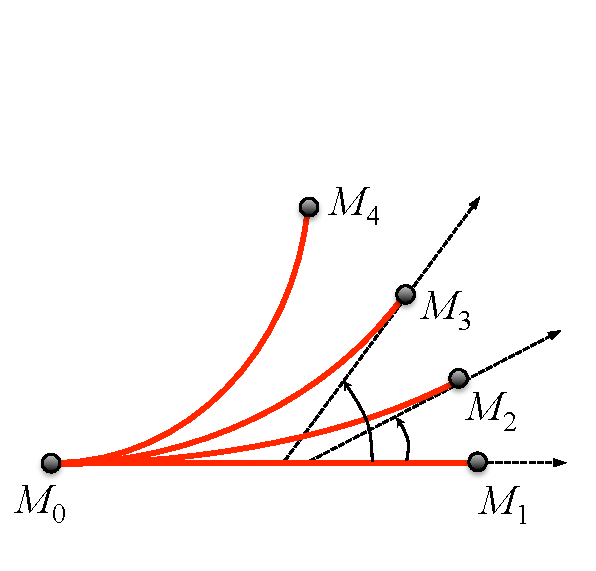
\includegraphics{./images/curves/c103.pdf}}}

				\vspace{-1em}\invisible<1->{{\b 长度相同的曲线,切线

				转角越大弯曲程度越大}}
			\end{center}
		\column{.5\textwidth}
	\end{columns}
\end{frame}

\begin{frame}{曲率}
	\linespread{1.2}
	\centerline{\ba{如何刻画曲线的弯曲程度?}}

	\begin{columns}
		\column{.5\textwidth}
			\begin{center}
				\vspace{-1em}
				{\resizebox{!}{5.5cm}{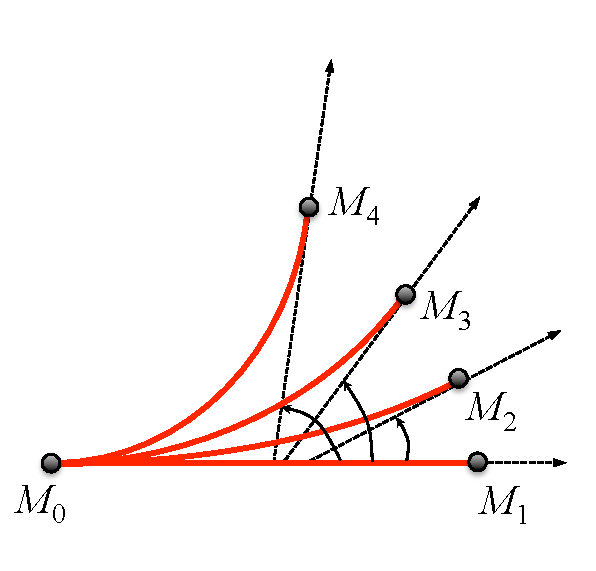
\includegraphics{./images/curves/c102.pdf}}}

				\vspace{-1em}\invisible<1->{{\b 长度相同的曲线,切线

				转角越大弯曲程度越大}}
			\end{center}
		\column{.5\textwidth}
	\end{columns}
\end{frame}

\begin{frame}{曲率}
	\linespread{1.2}
	\centerline{\ba{如何刻画曲线的弯曲程度?}}

	\begin{columns}
		\column{.5\textwidth}
			\begin{center}
				\vspace{-1em}
				{\resizebox{!}{5.5cm}{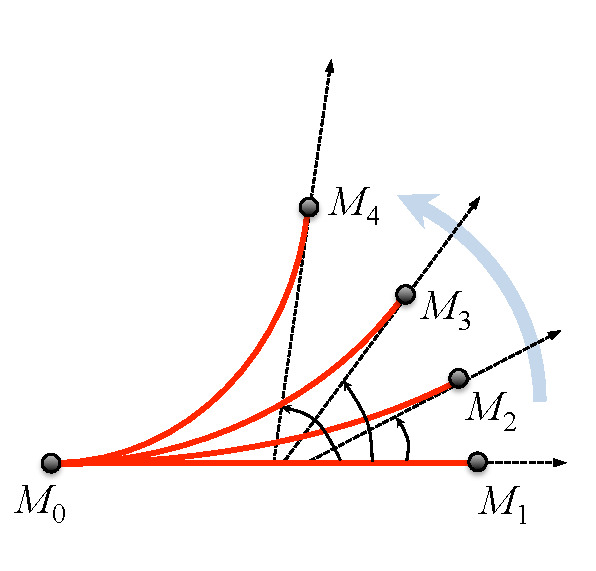
\includegraphics{./images/curves/c101.pdf}}}

				\vspace{-1em}{{\b 长度相同的曲线,切线

				转角越大弯曲程度越大}}
			\end{center}
		\column{.5\textwidth}
	\end{columns}
\end{frame}

% \begin{frame}{曲率}
% 	\linespread{1.2}
% 	\centerline{\ba{如何刻画曲线的弯曲程度?}}
% 
% 	\begin{columns}
% 		\column{.5\textwidth}
% 			\begin{center}
% 				\vspace{-1em}
% 				{\resizebox{!}{5.5cm}{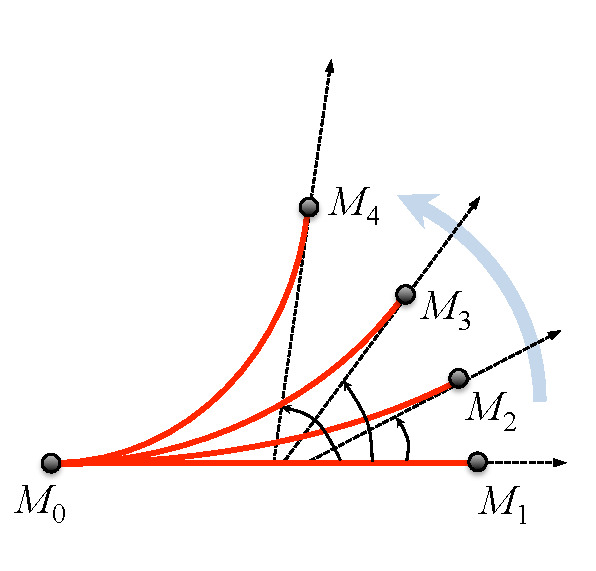
\includegraphics{./images/curves/c101.pdf}}}
% 
% 				\vspace{-1em}{{\b 长度相同的曲线,切线
% 				
% 				转角越大弯曲程度越大}}	
% 			\end{center}
% 		\column{.5\textwidth}
% 			\begin{center}			
% 				\vspace{-1em}
% 				{\resizebox{!}{5.5cm}{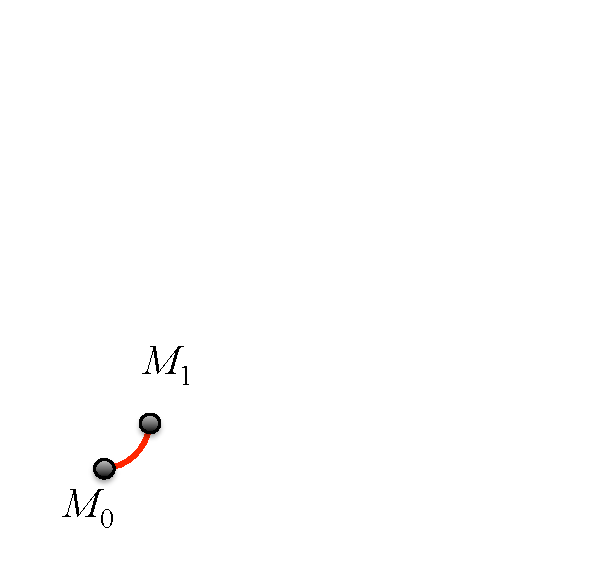
\includegraphics{./images/curves/c208.pdf}}}
% 				
% 				\vspace{-1em}{\color{white} 切线转角相同的曲线,
% 
% 				弧长越短弯曲程度越大}
% 			\end{center}
% 	\end{columns}
% \end{frame}
% 
% \begin{frame}{曲率}
% 	\linespread{1.2}
% 	\centerline{\ba{如何刻画曲线的弯曲程度?}}
% 
% 	\begin{columns}
% 		\column{.5\textwidth}
% 			\begin{center}
% 				\vspace{-1em}
% 				{\resizebox{!}{5.5cm}{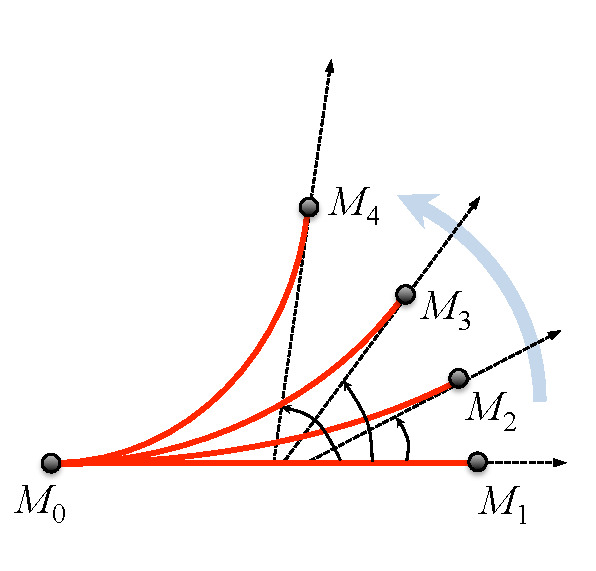
\includegraphics{./images/curves/c101.pdf}}}
% 
% 				\vspace{-1em}{{\b 长度相同的曲线,切线
% 
% 				转角越大弯曲程度越大}}
% 			\end{center}
% 		\column{.5\textwidth}
% 			\begin{center}
% 				\vspace{-1em}
% 				{\resizebox{!}{5.5cm}{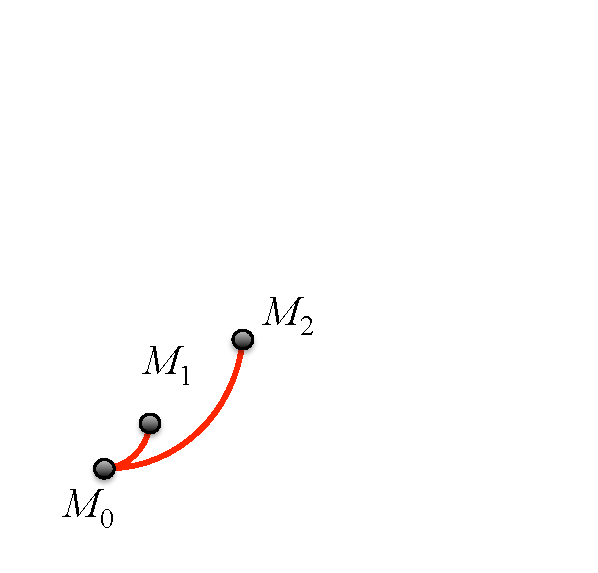
\includegraphics{./images/curves/c207.pdf}}}
% 				
% 				\vspace{-1em}{\color{white} 切线转角相同的曲线,
% 
% 				弧长越短弯曲程度越大}
% 			\end{center}
% 	\end{columns}
% \end{frame}

\begin{frame}{曲率}
	\linespread{1.2}
	\centerline{\ba{如何刻画曲线的弯曲程度?}}

	\begin{columns}
		\column{.5\textwidth}
			\begin{center}
				\vspace{-1em}
				{\resizebox{!}{5.5cm}{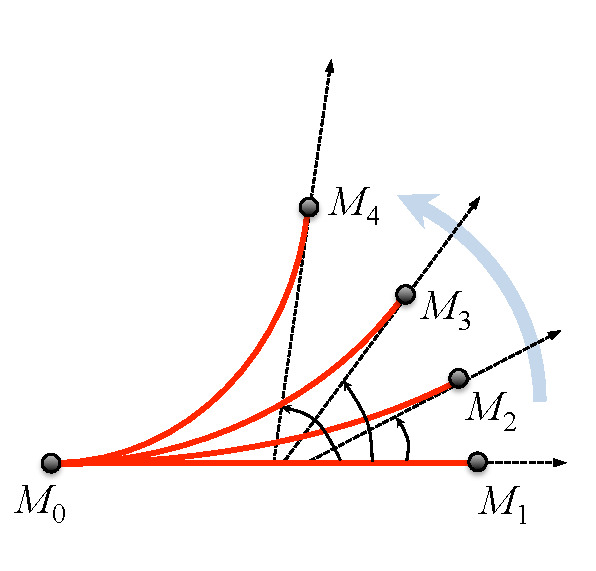
\includegraphics{./images/curves/c101.pdf}}}

				\vspace{-1em}{{\b 长度相同的曲线,切线

				转角越大弯曲程度越大}}
			\end{center}
		\column{.5\textwidth}
			\begin{center}
				\vspace{-1em}
				{\resizebox{!}{5.5cm}{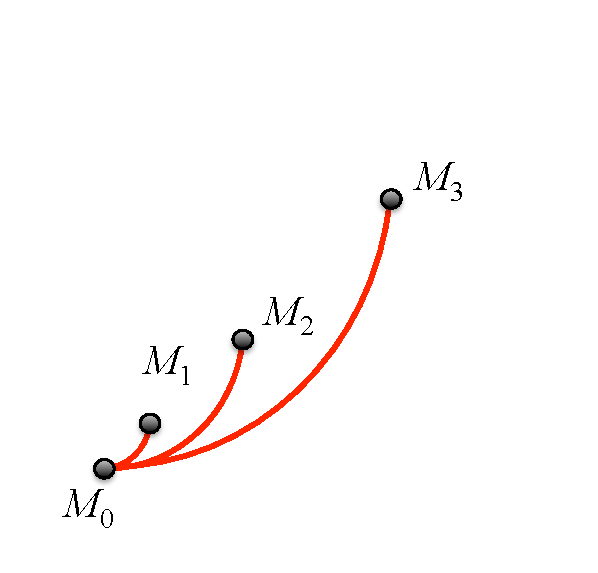
\includegraphics{./images/curves/c206.pdf}}}
				
				\vspace{-1em}{\color{white} 切线转角相同的曲线,

				弧长越短弯曲程度越大}
			\end{center}
	\end{columns}
\end{frame}

\begin{frame}{曲率}
	\linespread{1.2}
	\centerline{\ba{如何刻画曲线的弯曲程度?}}

	\begin{columns}
		\column{.5\textwidth}
			\begin{center}
				\vspace{-1em}
				{\resizebox{!}{5.5cm}{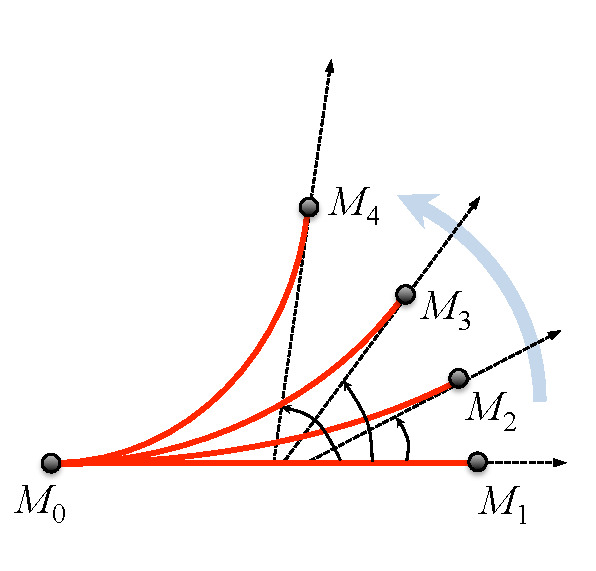
\includegraphics{./images/curves/c101.pdf}}}

				\vspace{-1em}{{\b 长度相同的曲线,切线

				转角越大弯曲程度越大}}
			\end{center}
		\column{.5\textwidth}
			\begin{center}
				\vspace{-1em}
				{\resizebox{!}{5.5cm}{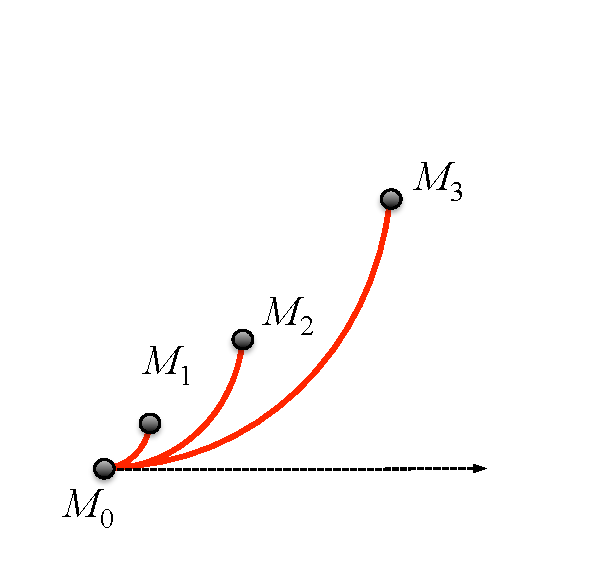
\includegraphics{./images/curves/c205.pdf}}}
				
				\vspace{-1em}{\color{white} 切线转角相同的曲线,

				弧长越短弯曲程度越大}
			\end{center}
	\end{columns}
\end{frame}

\begin{frame}{曲率}
	\linespread{1.2}
	\centerline{\ba{如何刻画曲线的弯曲程度?}}

	\begin{columns}
		\column{.5\textwidth}
			\begin{center}
				\vspace{-1em}
				{\resizebox{!}{5.5cm}{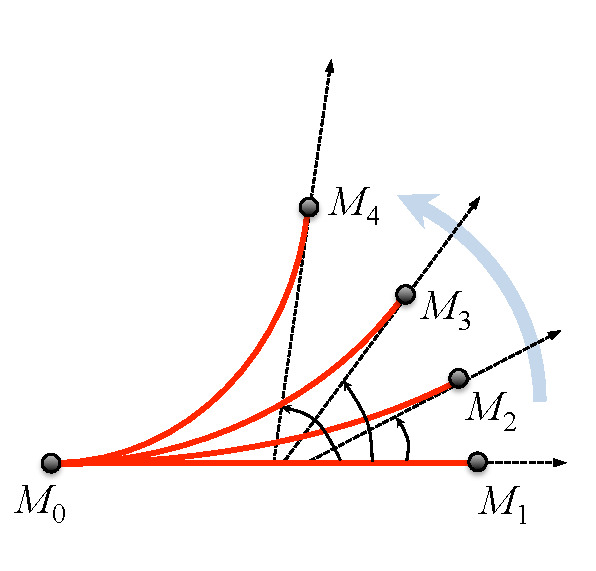
\includegraphics{./images/curves/c101.pdf}}}

				\vspace{-1em}{{\b 长度相同的曲线,切线

				转角越大弯曲程度越大}}
			\end{center}
		\column{.5\textwidth}
			\begin{center}
				\vspace{-1em}
				{\resizebox{!}{5.5cm}{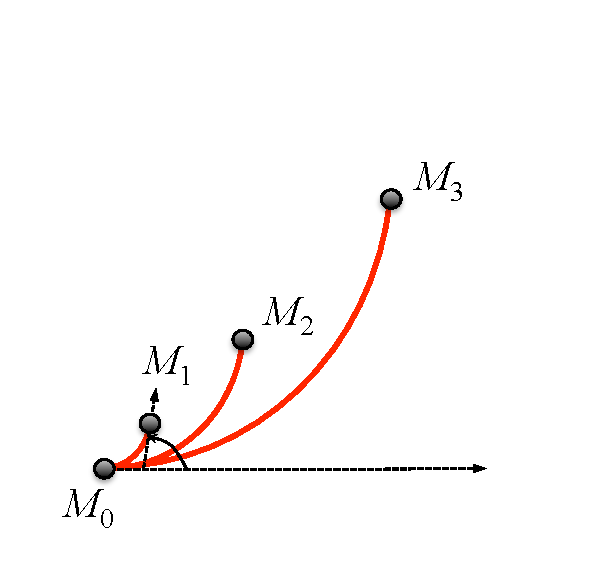
\includegraphics{./images/curves/c204.pdf}}}
				
				\vspace{-1em}{\color{white} 切线转角相同的曲线,

				弧长越短弯曲程度越大}
			\end{center}
	\end{columns}
\end{frame}

\begin{frame}{曲率}
	\linespread{1.2}
	\centerline{\ba{如何刻画曲线的弯曲程度?}}

	\begin{columns}
		\column{.5\textwidth}
			\begin{center}
				\vspace{-1em}
				{\resizebox{!}{5.5cm}{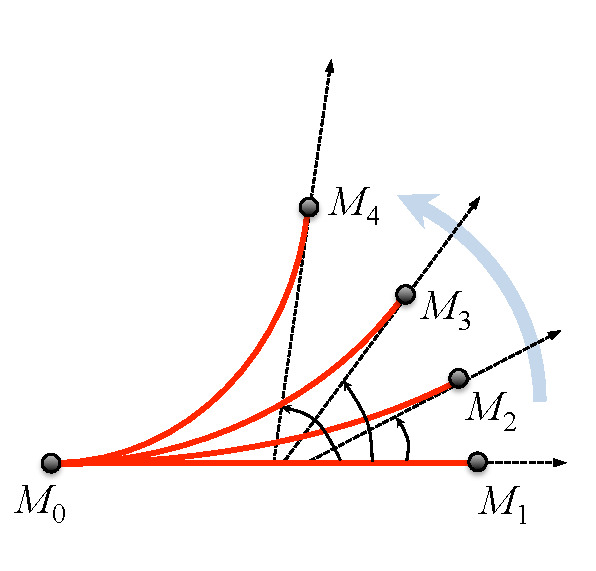
\includegraphics{./images/curves/c101.pdf}}}

				\vspace{-1em}{{\b 长度相同的曲线,切线

				转角越大弯曲程度越大}}
			\end{center}
		\column{.5\textwidth}
			\begin{center}
				\vspace{-1em}
				{\resizebox{!}{5.5cm}{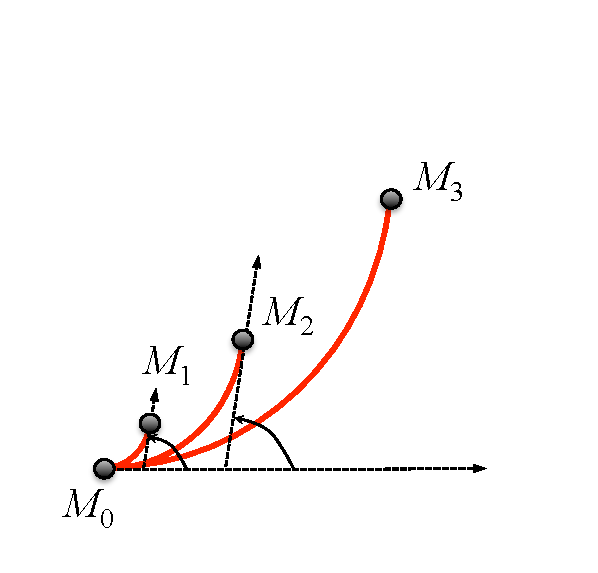
\includegraphics{./images/curves/c203.pdf}}}
				
				\vspace{-1em}{\color{white} 切线转角相同的曲线,

				弧长越短弯曲程度越大}
			\end{center}
	\end{columns}
\end{frame}

\begin{frame}{曲率}
	\linespread{1.2}
	\centerline{\ba{如何刻画曲线的弯曲程度?}}

	\begin{columns}
		\column{.5\textwidth}
			\begin{center}
				\vspace{-1em}
				{\resizebox{!}{5.5cm}{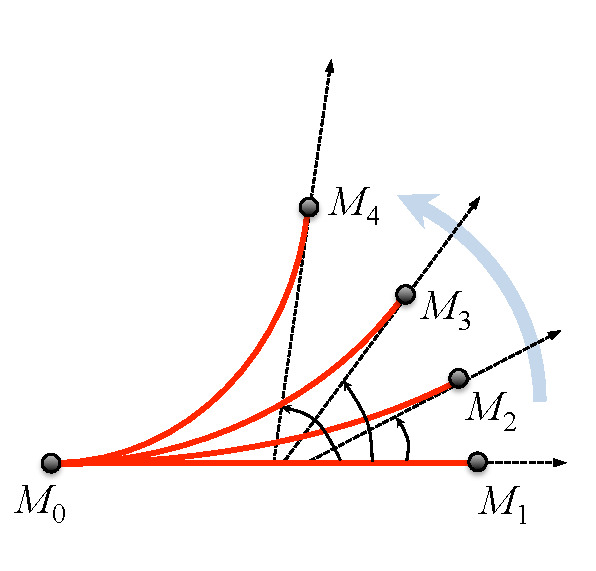
\includegraphics{./images/curves/c101.pdf}}}

				\vspace{-1em}{{\b 长度相同的曲线,切线

				转角越大弯曲程度越大}}
			\end{center}
		\column{.5\textwidth}
			\begin{center}
				\vspace{-1em}
				{\resizebox{!}{5.5cm}{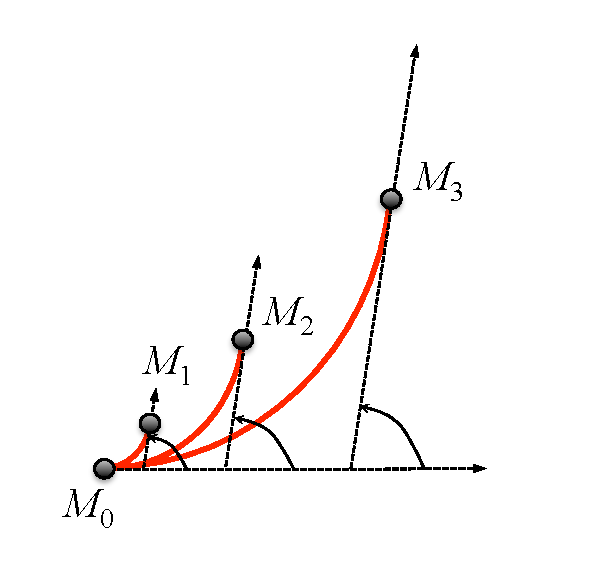
\includegraphics{./images/curves/c202.pdf}}}
				
				\vspace{-1em}{\color{white} 切线转角相同的曲线,

				弧长越短弯曲程度越大}
			\end{center}
	\end{columns}
\end{frame}

\begin{frame}{曲率}
	\linespread{1.2}
	\centerline{\ba{如何刻画曲线的弯曲程度?}}

	\begin{columns}
		\column{.5\textwidth}
			\begin{center}
				\vspace{-1em}
				{\resizebox{!}{5.5cm}{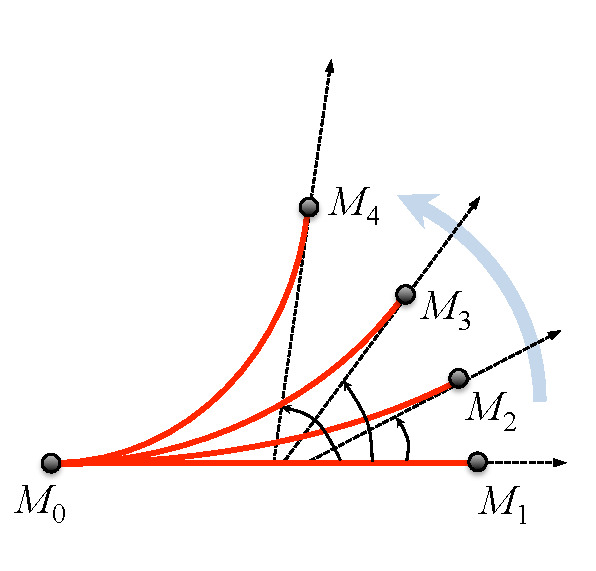
\includegraphics{./images/curves/c101.pdf}}}

				\vspace{-1em}{{\b 长度相同的曲线,切线

				转角越大弯曲程度越大}}
			\end{center}
		\column{.5\textwidth}
			\begin{center}
				\vspace{-1em}
				{\resizebox{!}{5.5cm}{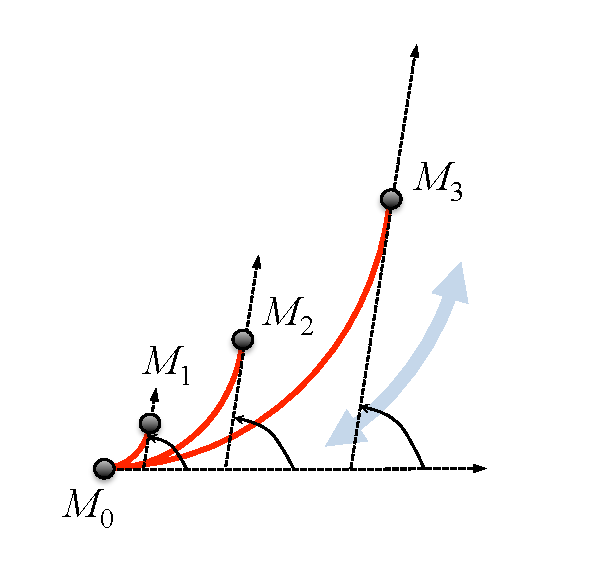
\includegraphics{./images/curves/c201.pdf}}}
				
				\vspace{-1em}{\b 切线转角相同的曲线,

				弧长越短弯曲程度越大}
			\end{center}
	\end{columns}
\end{frame}

%=================================================

\begin{frame}{1、曲率的定义}
	\linespread{1.5}
	\ba{曲线的弯曲程度与切线的转角成正比,与弧长成反比}\pause
	\begin{block}{{\bf 定义1}\hfill }
		设曲线$C$光滑且可求长度。\pause 从其上一点$M_0$出发,
		到另一点$M$的弧长
		为$\Delta s$,切线转角为$\Delta\alpha$。
		\pause 若极限$\lim\limits_{\Delta s\to
		0}\left|\df{\Delta\alpha}{\Delta s}\right|$存在,
		则称之为{\bb 曲线$C$在$M_0$处的曲率:}
		
		\pause\vspace{-1em}
	$$\alert{K=\lim\limits_{\Delta s\to
				0}\left|\df{\Delta\alpha}{\Delta s}\right|\pause\pause
				=\left|\df{\d\alpha}{\d s}\right|}$$ 
	\end{block}\onslide<6->\vspace{-1ex}
	\begin{itemize}
	  \item \alert{在曲线上某一点处的切线转角关于弧长的变化率}
	\end{itemize}
\end{frame}

\subsection{曲率的计算}

\begin{frame}{2、曲率的计算}
	\linespread{1.2}\pause 
	\uncover<1-4,7->{设$y=f(x)$在$x_0$的某邻域内二阶可导,则
	\alert{$$K=\left|\df{\d\alpha}{\d s}\right|
				\pause =\df{|y''_{xx}|}{[1+(y'_x)^2]^{3/2}}$$}}\pause 
	\vspace{2em}
	\uncover<1-7>{\begin{exampleblock}{{\bf 例1}\hfill }
		求椭圆$x=3\cos t,y=2\sin t\,(0\leq t\leq 2\pi)$
		上任意点处的曲率,并指出其中曲率最大的点。
	\end{exampleblock}}
	\pause
	\begin{center}
		\onslide<6>\vspace{-7.5cm}{\resizebox{!}{4.5cm}{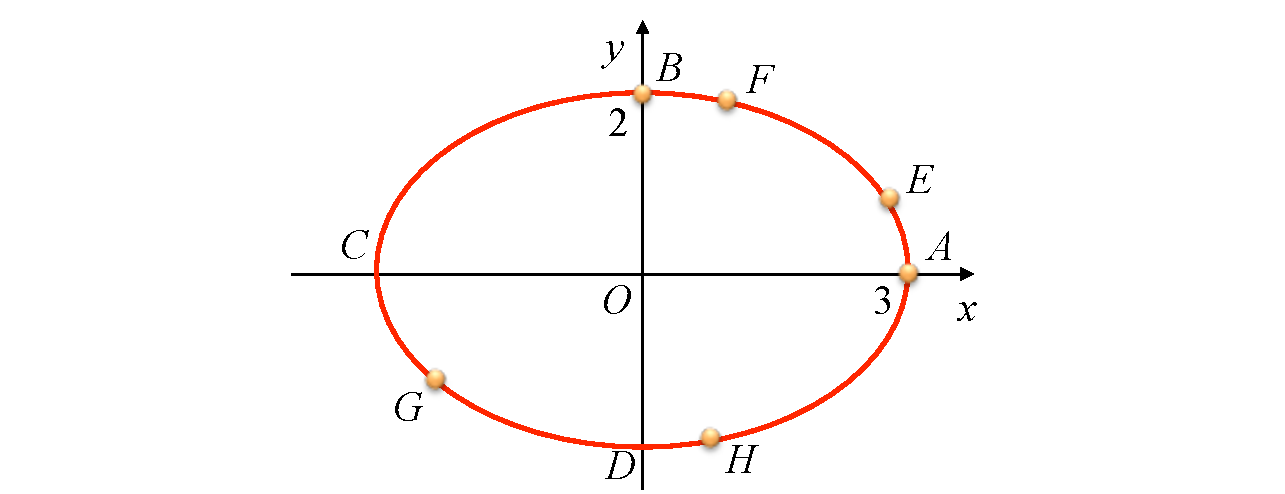
\includegraphics{./images/ec/newEC/ec01.pdf}}}
% 		\onslide<7>\vspace{-5.5cm}{\resizebox{!}{4.5cm}{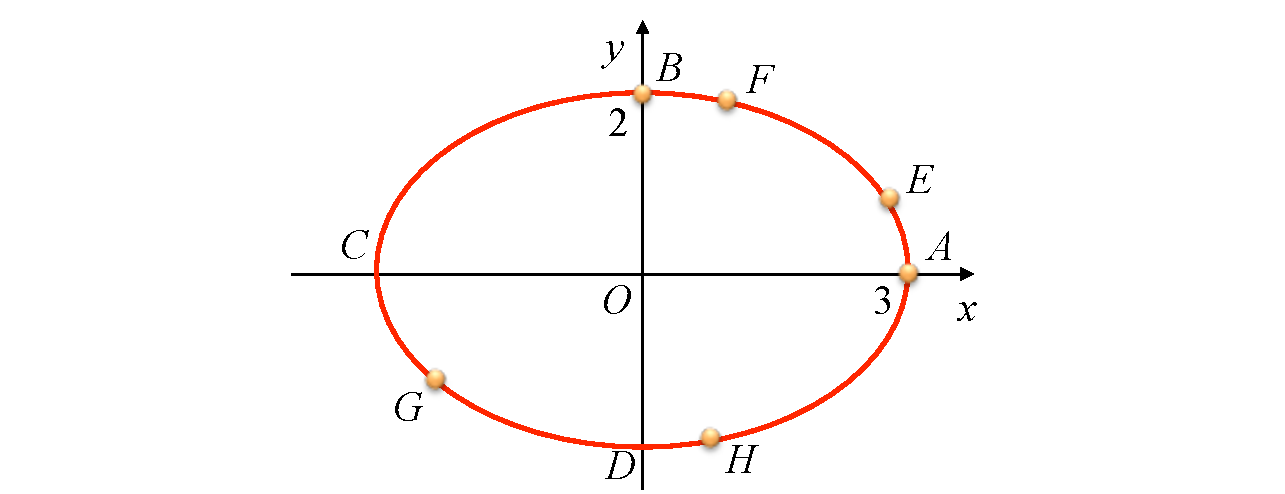
\includegraphics{./images/ec/newEC/ec01.pdf}}}
% 		\onslide<6>\vspace{-7.5cm}{\resizebox{!}{4.5cm}{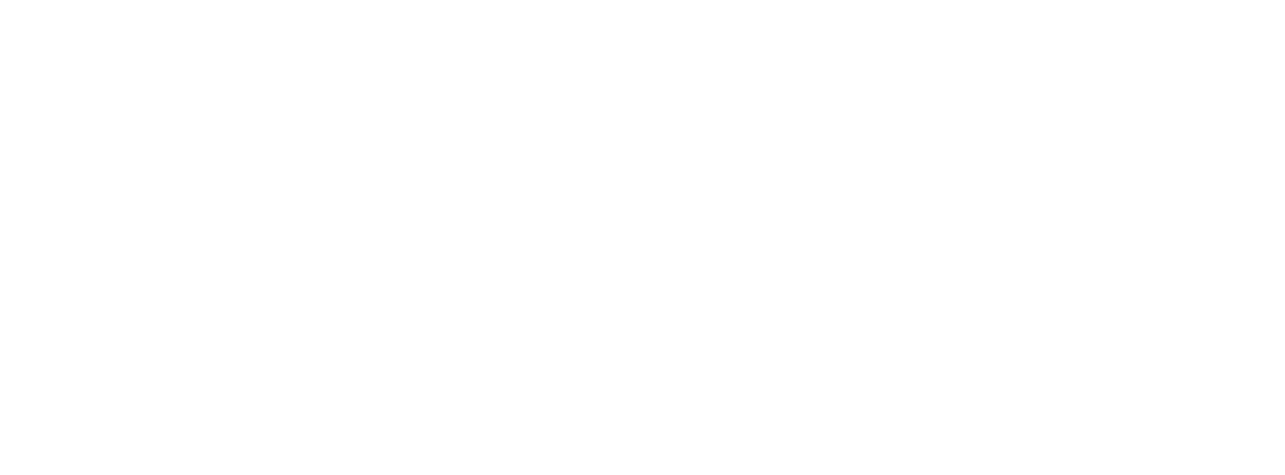
\includegraphics{./images/ec/newEC/ec00.pdf}}}%
% 		\vspace{-4.5cm}
% 		\only<7>{\resizebox{!}{4.5cm}{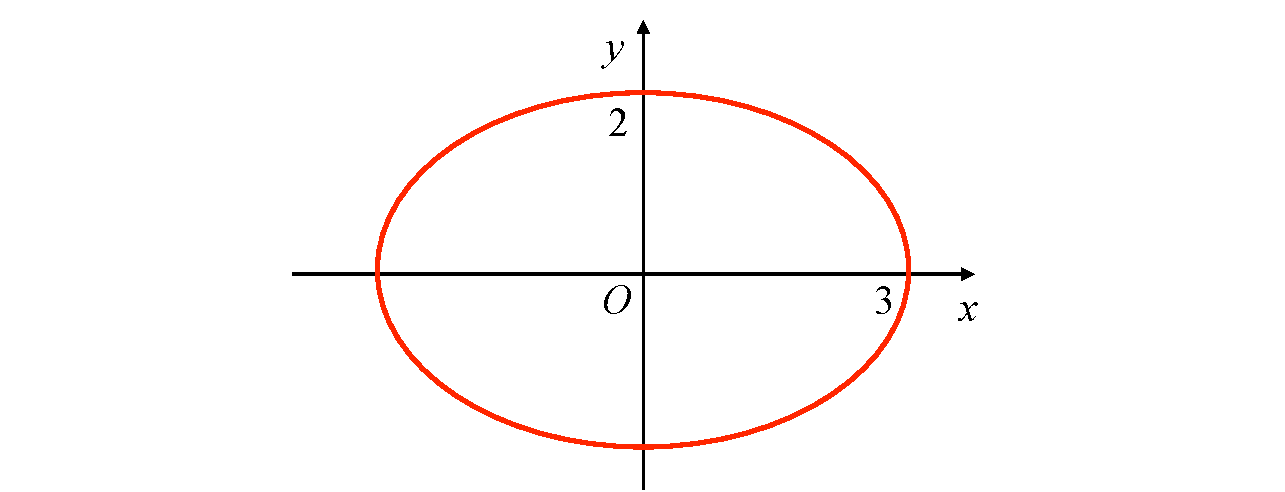
\includegraphics{./images/ec/newEC/ec07.pdf}}}%
	\end{center}
	\onslide<9->
	\vspace{-4em}
 	  {\bf 注:} {\b 参数方程下的曲率公式}
	  $$\alert{K=\df{|x'_ty''_{tt}-x''_{tt}y'_t|}
		{\{[x'_t]^2+[y'_t]^2\}^{3/2}}}$$
% 	  \bigskip\bigskip
	  \onslide<10>\ba{思考:}{\b 如何给出极坐标下的曲率公式?}
\end{frame}

\subsection{曲率圆与曲率的应用}

% \begin{frame}{3、曲率圆与曲率的应用}
% 	\linespread{1.2} \pause 
% 	{\bb 曲率圆:}与给定曲线在凹侧相切,且曲率相同的圆
% 	
% 	\pause\vspace{1ex}
% 	\begin{center}
% 		\resizebox{!}{4cm}{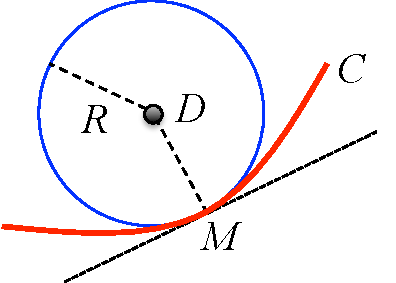
\includegraphics{./images/curSphere.pdf}}
% 	\end{center}
% 	\vspace{-1em}\pause 
% 	\begin{block}{\bf 定理1}
% 		曲率圆与给定曲线二阶相切。
% 	\end{block}
% \end{frame}

\begin{frame}{3、曲率圆与曲率的应用}
	\linespread{1.2} \pause 
	{\bb 曲率圆:}与给定曲线在凹侧相切,且曲率相同的圆
	
	\pause\vspace{1ex}
	\begin{columns}
		\column{.55\textwidth}
			\begin{center}
				\resizebox{!}{4cm}{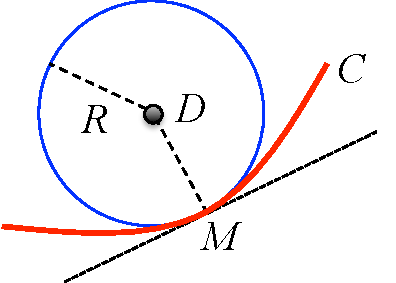
\includegraphics{./images/curSphere.pdf}}
			\end{center}
		\column{.45\textwidth}
			\uncover<5->{{\bf 思考:}与已知曲线在给定点处二阶相切的圆一定是其曲率圆吗?}
			\uncover<6->{$\alert{\bm{\surd}}$}
	\end{columns}
	
% 	\vspace{-1em}
	\pause 
	\begin{block}{\bf 定理1}
		曲率圆与给定曲线二阶相切。
	\end{block}
\end{frame}

\begin{frame}
	\linespread{1.2} 
	\begin{exampleblock}{{\bf 例2}(加工问题)\hfill }
		已知某工件内侧的截痕曲线为椭圆$\df{x^2}9+\df{y^2}4=1$,
		若用圆形砂轮对其进行打磨,问该如何选择砂轮的尺寸?
	\end{exampleblock}
	\vspace{-1em}
	\begin{columns}
		\column{.55\textwidth}
			\begin{center}
				\only<1>{\resizebox{!}{5.5cm}{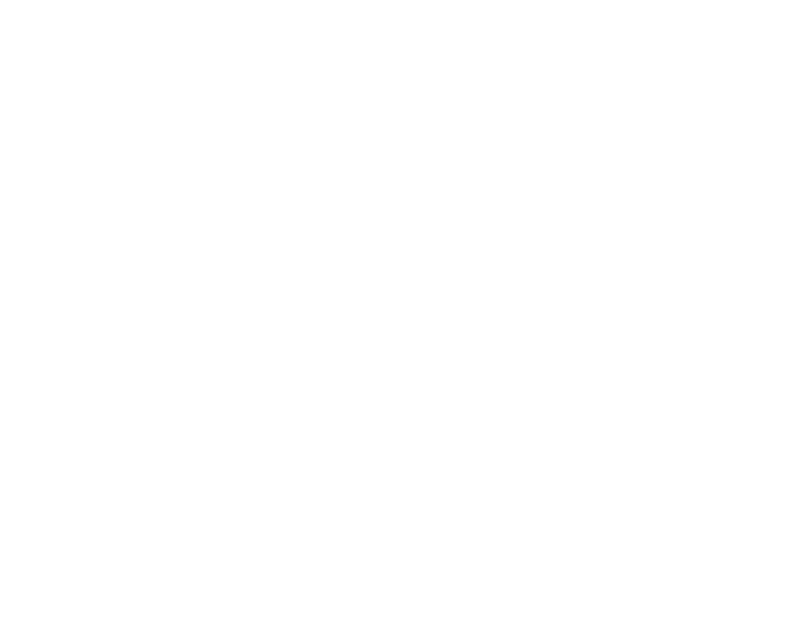
\includegraphics{./images/SE/S0x.pdf}}}%
				\only<2>{\resizebox{!}{5.5cm}{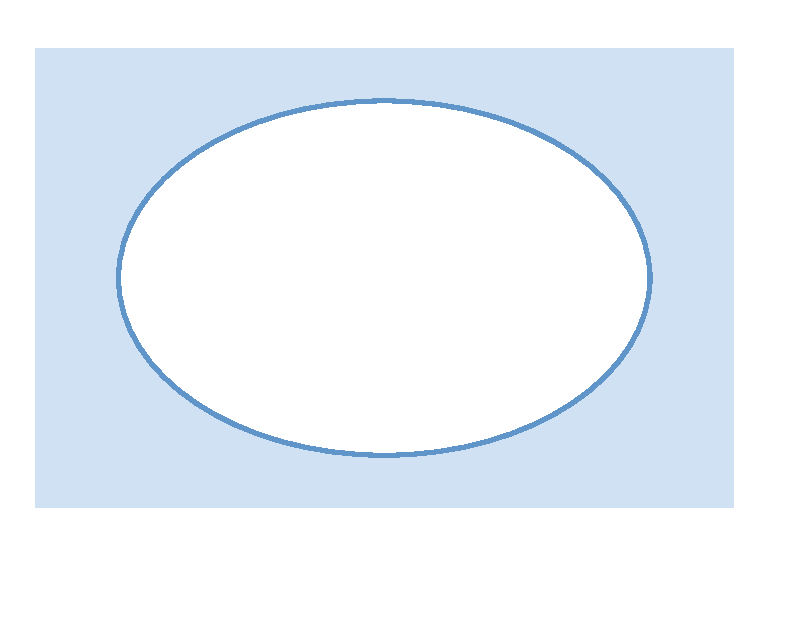
\includegraphics{./images/SE/S05.pdf}}}%
				\only<3-4>{\resizebox{!}{5.5cm}{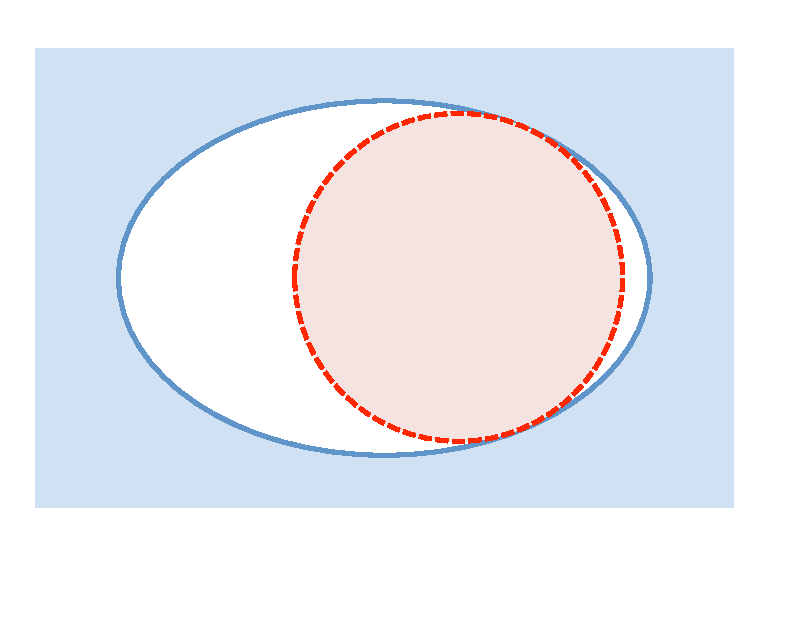
\includegraphics{./images/SE/S04.pdf}}}%
				\only<5-6>{\resizebox{!}{5.5cm}{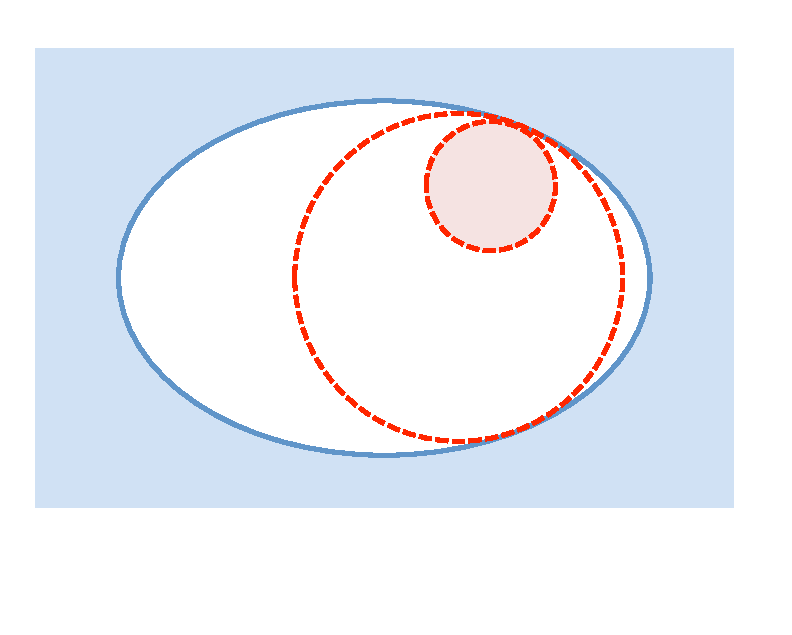
\includegraphics{./images/SE/S03.pdf}}}%
				\only<7-8>{\resizebox{!}{5.5cm}{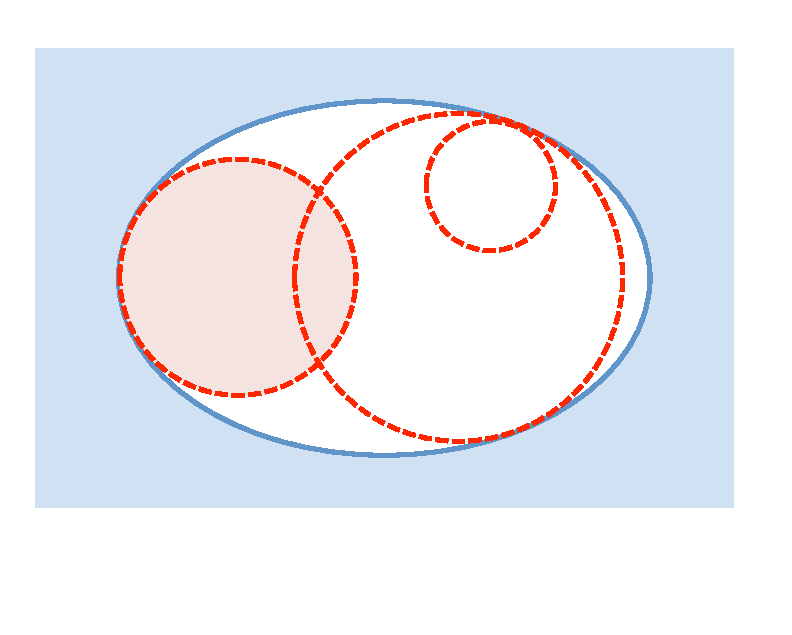
\includegraphics{./images/SE/S02.pdf}}}%
				\only<9>{\resizebox{!}{5.5cm}{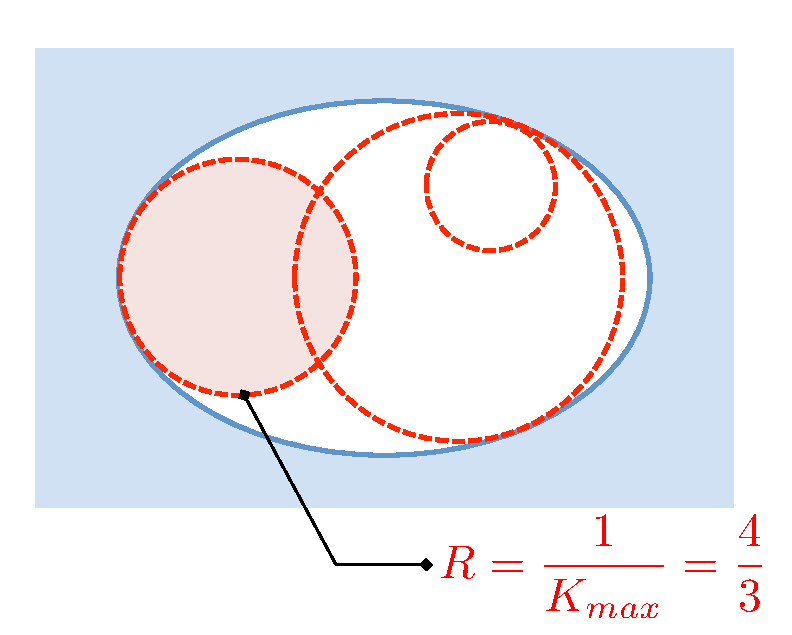
\includegraphics{./images/SE/S01.pdf}}}%
			\end{center}
		\column{.45\textwidth}
			\begin{itemize}
			  \item<4-> 半径过大$\Rightarrow$无法完全打磨
			  \item<6-> 半径过小$\Rightarrow$打磨效率过低
			  \item<8-> {\bf 最优解:}\alert{半径最小的曲率圆}
			\end{itemize}
	\end{columns}
\end{frame}

\begin{frame}{曲率半径与离心力}
	\linespread{1.2}
	\begin{columns}
		\column{.6\textwidth}
			质量为$m$的质点以速度$v$通过光滑曲线上一点,所受离心力为
			$$F=\df{mv^2}{R},$$
			其中$R$为曲线在该点处的曲率半径。
		\column{.4\textwidth}
			\begin{center}
				\resizebox{!}{4.5cm}{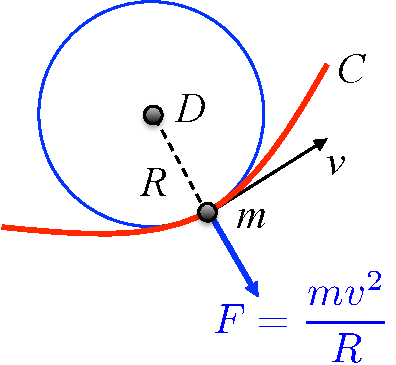
\includegraphics{./images/flip.pdf}}
			\end{center}
	\end{columns}
\end{frame}

\begin{frame}{铁路中的缓和曲线}
	\linespread{1.2}\pause
	\begin{columns}
		\column{.2\textwidth}
			\begin{center}
				\resizebox{!}{1.2cm}{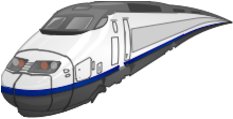
\includegraphics{./images/train.pdf}}
			\end{center}
		\column{.8\textwidth}
			\ba{为了确保列车行驶安全,尽可能保证列车运行时所受离心力的平稳变化。}\pause 
	\end{columns} 
	\vspace{-1em}
	\begin{columns}
		\column{.65\textwidth}
			\begin{center}
				\only<1-2>{\resizebox{!}{5.5cm}{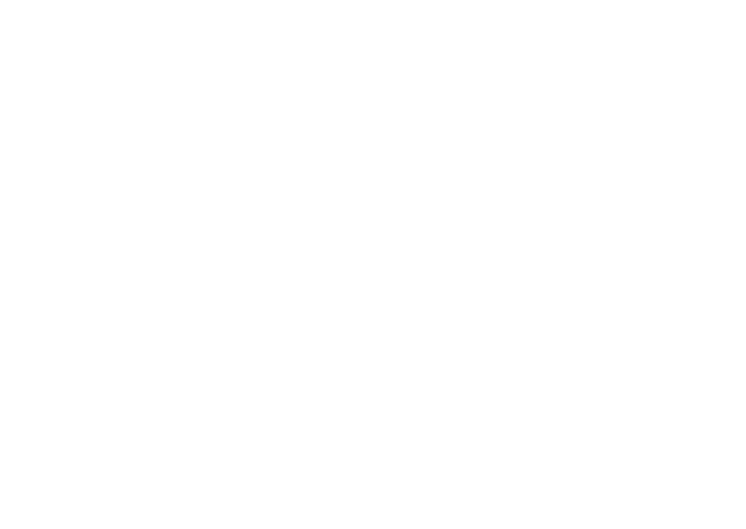
\includegraphics{./images/rc00.pdf}}}%
				\only<3-8>{\resizebox{!}{5.5cm}{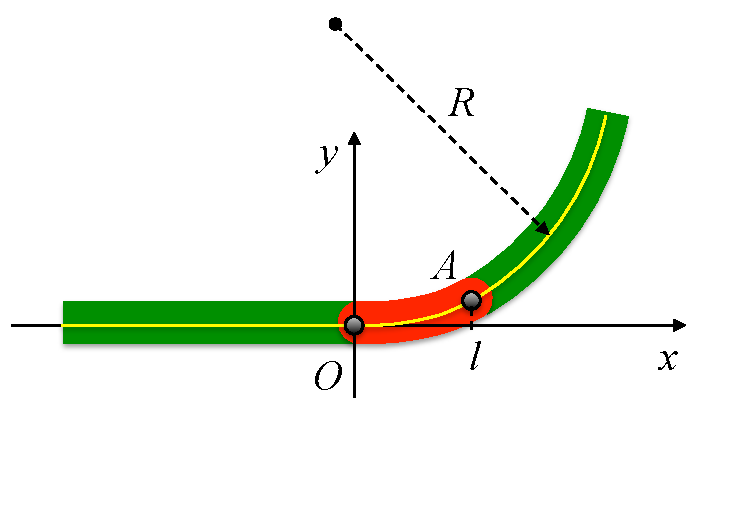
\includegraphics{./images/rc02.pdf}}}%
			\end{center}
		\column{.35\textwidth}
			\uncover<4->{\ba{常用的缓和曲线:}}%
			\begin{itemize}
			  \item<5-> {\b 三次多项式}
			  \item<6-> {\b 渐开螺旋线}
			  \item<7-> {\b 双扭线}
			  \item<8-> {\b \ldots}
			\end{itemize}
	\end{columns}
\end{frame}

\begin{frame}
	\linespread{1.2}
	\begin{exampleblock}{{\bf 例3}(铁路的缓和曲线)}
		如图,列车匀速行进,经过一段直线轨道后,将进入半径为$R$的圆弧轨道。为
		尽量减少列车行驶中所受的离心力冲击,
		试确定一个三次多项式函数实现两段轨道的连接。
	\end{exampleblock}
	\vspace{-1ex}
	\begin{center}
		\only<1>{\resizebox{!}{5.2cm}{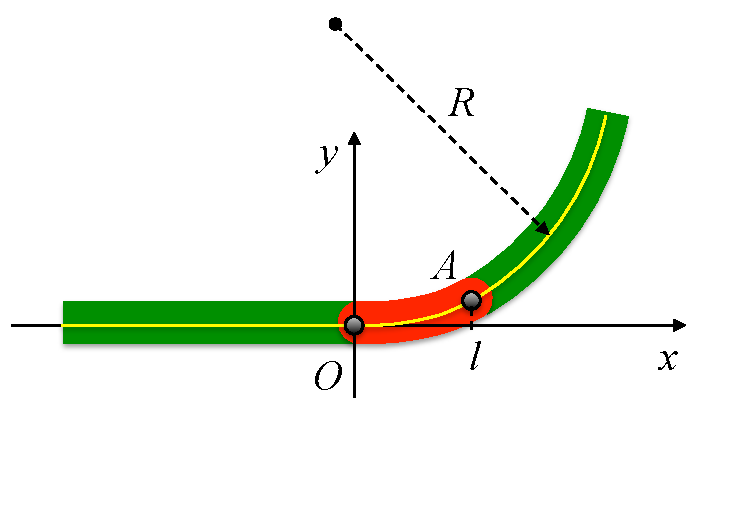
\includegraphics{./images/rc02.pdf}}}%
		\only<2>{\resizebox{!}{5.2cm}{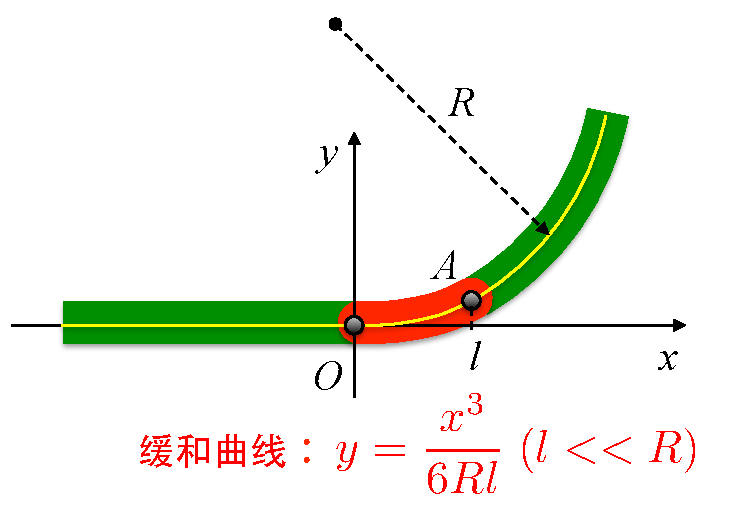
\includegraphics{./images/rc01.pdf}}}%
	\end{center}
\end{frame}

\begin{frame}
	\linespread{1}
	\begin{columns}
		\column{.55\textwidth}
			\resizebox{!}{4.5cm}{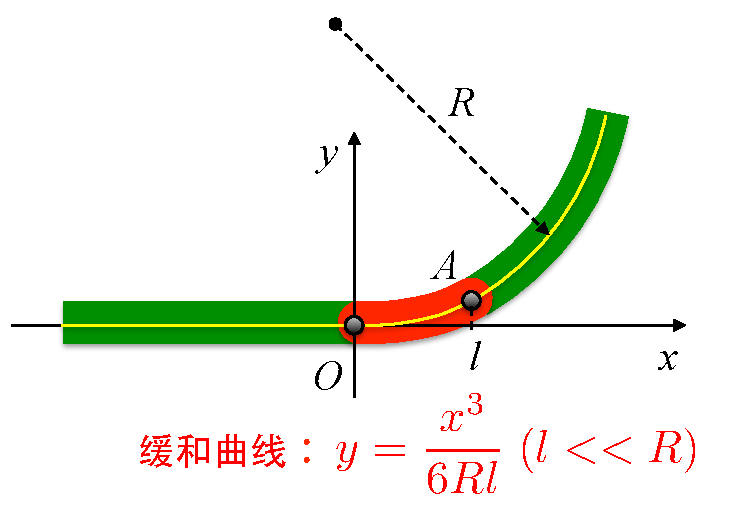
\includegraphics{./images/rc01.pdf}}\pause
		\column{.45\textwidth}
			{\small
			\begin{itemize}
			  \item 匀速行驶$v=108km/h$\pause
			  \item 列车重量$m=500t$\pause
			  \item 圆弧半径$R=1000m$\pause
			  \item 缓和曲线长$l=90m$
			\end{itemize}
			}
	\end{columns}
	\vspace{-1em}\pause
	\begin{columns}
		\column{.55\textwidth}
			\begin{center}
				\resizebox{!}{4cm}{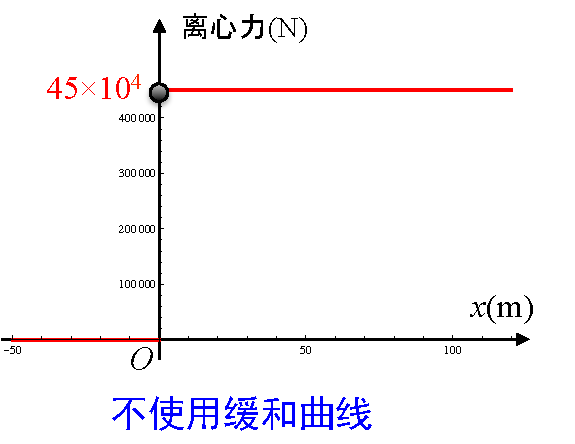
\includegraphics{./images/f01.pdf}}\pause
			\end{center}
		\column{.45\textwidth}
			\begin{center}
				\resizebox{!}{4cm}{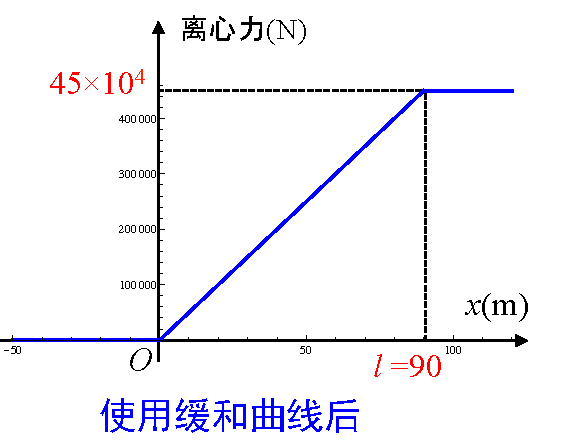
\includegraphics{./images/f02.pdf}}
			\end{center}
	\end{columns}
\end{frame}

\begin{frame}{铁路与轨道交通}
	\linespread{1.2}
	\vspace{-2em}
	\begin{center}
		\hspace{1em}\resizebox{!}{8cm}{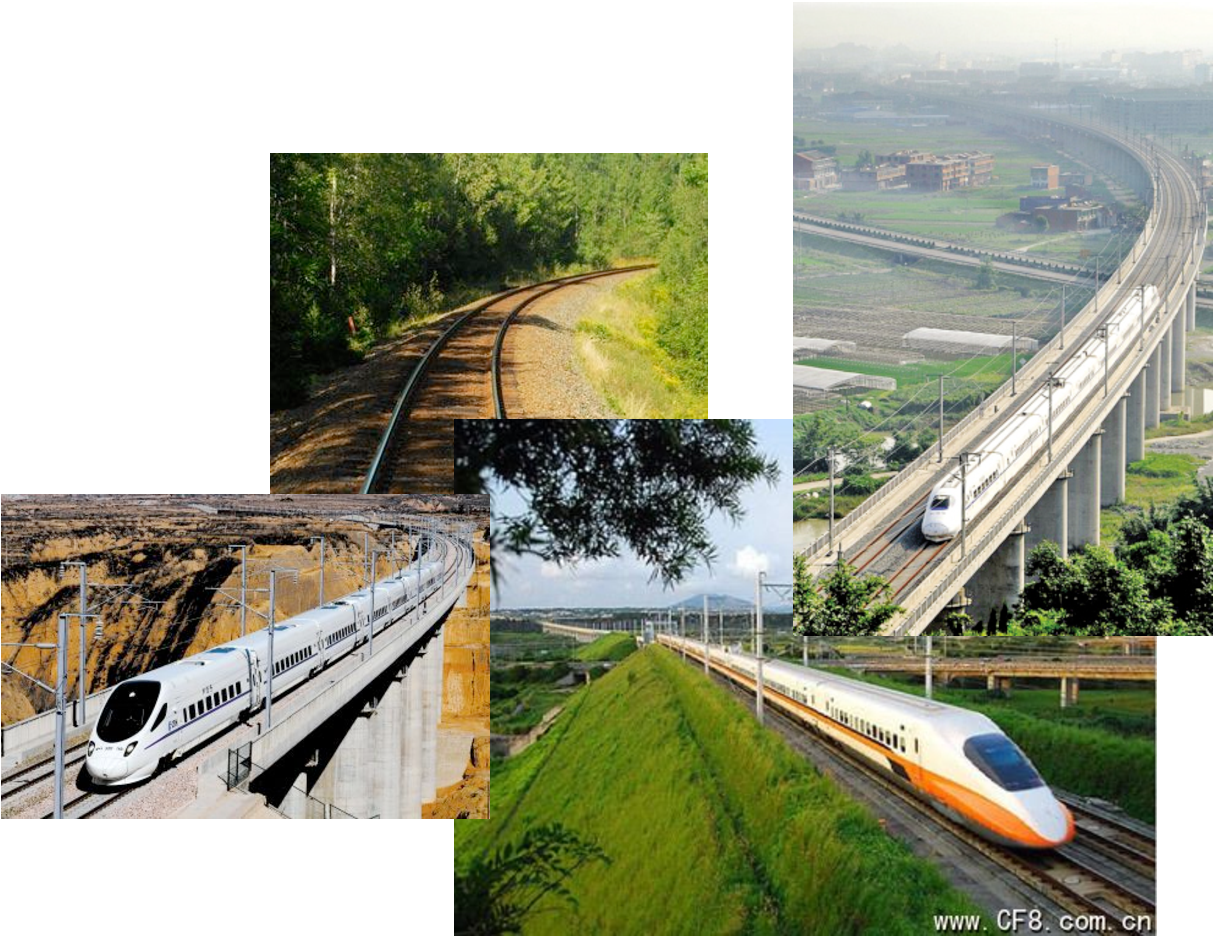
\includegraphics{./images/hr.pdf}}
	\end{center}
\end{frame}

\begin{frame}{高速公路}
	\linespread{1.2}
	\vspace{-1ex}
	\begin{center}
		\hspace{1em}\resizebox{!}{7.2cm}{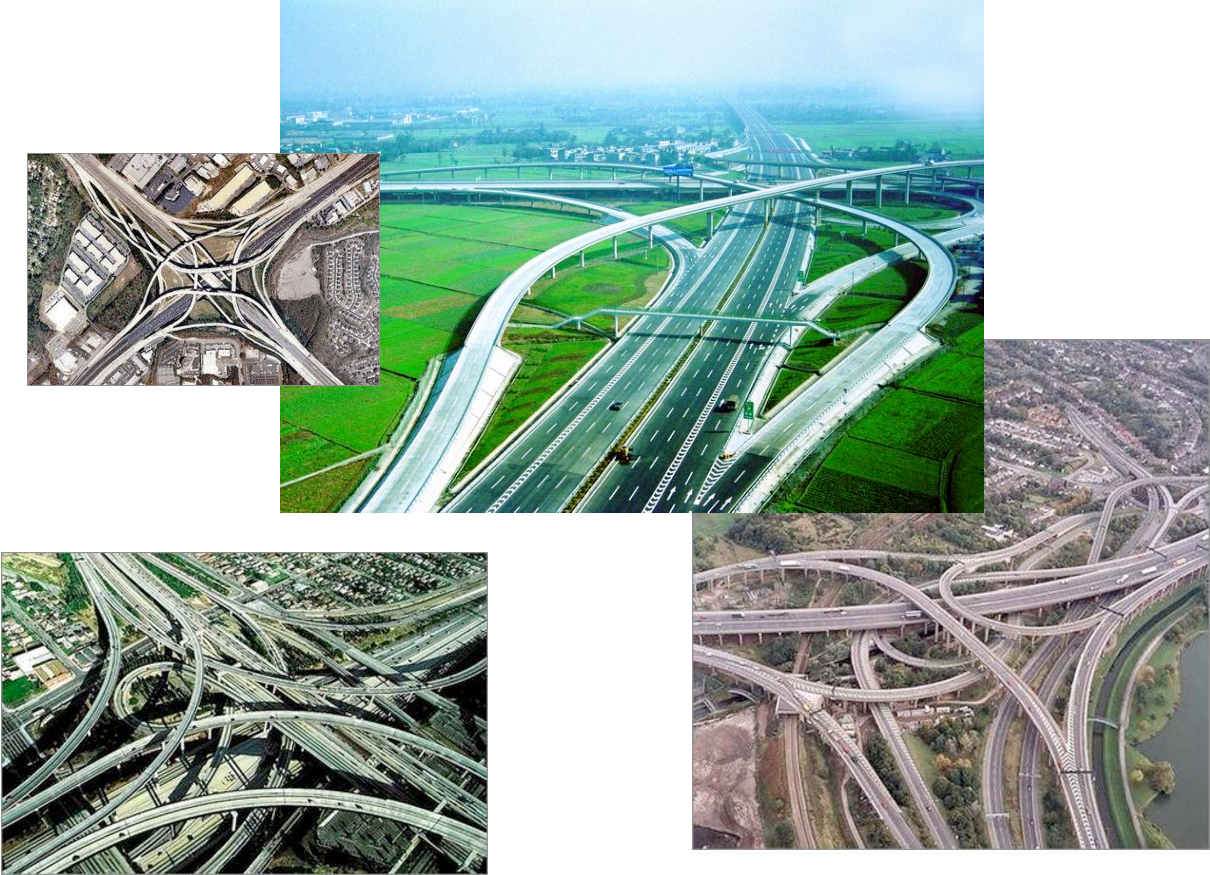
\includegraphics{./images/hw.pdf}}
	\end{center}
\end{frame}

\begin{frame}{过山车}
	\linespread{1.2}
	\vspace{-1ex}
	\begin{center}
		\hspace{1em}\resizebox{!}{7cm}{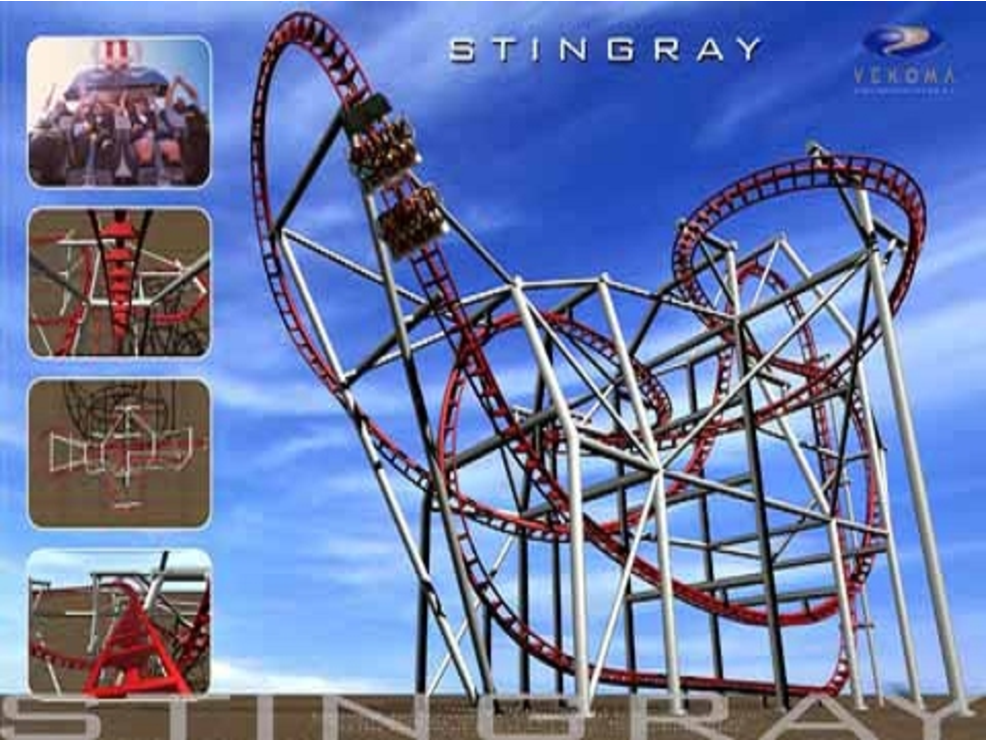
\includegraphics{./images/stg01.pdf}}
	\end{center}
\end{frame}

\begin{frame}{过山车}
	\linespread{1.2}
	\vspace{-1ex}
	\begin{center}
		\hspace{1em}\resizebox{!}{7.2cm}{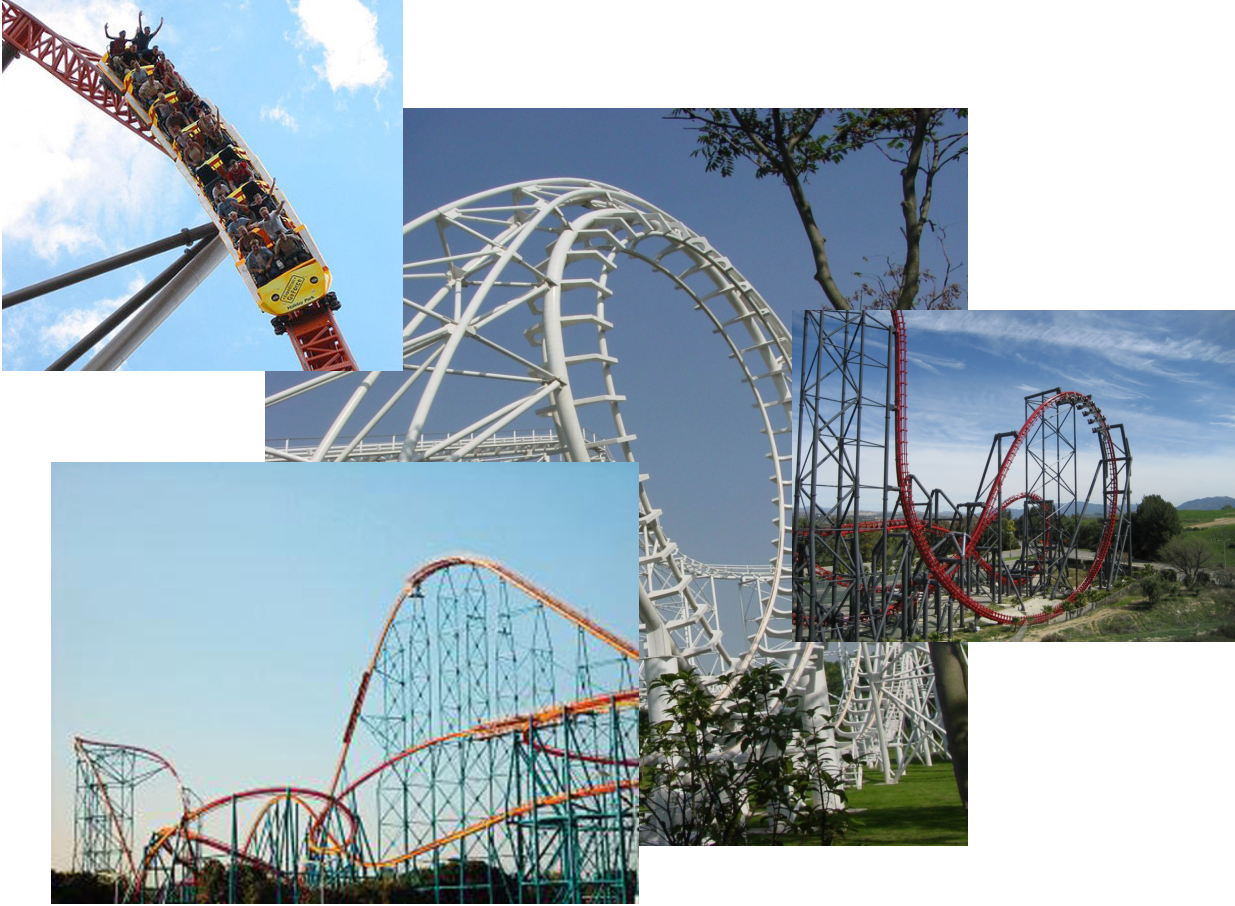
\includegraphics{./images/stg02.pdf}}
	\end{center}
\end{frame}

\begin{frame}{小结}
	\linespread{1.2}
	\begin{enumerate}
	  \item {\bf 曲率:}切线转角相对于弧长的变化率
	  \item {\bf 曲率的计算:}
	  $$\alert{K=\left|\df{\d\alpha}{\d s}\right|
				=\df{|y''_{xx}|}{[1+(y'_x)^2]^{3/2}}}$$
% 	  \begin{itemize}
% 	    \item 参数方程形式的曲率公式
% 	  \end{itemize}
	  \item {\bf 曲率圆与曲率的应用}
	  \begin{itemize}
	    \item 曲率半径、离心力与缓和曲线
	  \end{itemize}
	\end{enumerate}
	\pause
	\begin{exampleblock}{{\bf 课后思考题}(过山车设计)\hfill}
		试设计一个分段的多项式函数,完成过山车上两段不同斜率的直线轨道的接合。
	\end{exampleblock}
\end{frame}

% \begin{frame}{课后思考}
% 	\linespread{1.2}
% 	在{\bb 过山车的设计}中,必须遵从所谓的
% 	\begin{exampleblock}{{\bf 课后思考题}(过山车设计)\hfill}
% 		试设计一个分段的多项式函数,完成过山车上一段水平轨道与一段上坡直线轨道的接合。
% 	\end{exampleblock}
% \end{frame}
